% =====================================================================
%  ncwu_beamer_huashui_blue
%  来源：三大中值定理及其应用课件（华水蓝，原 27 帧）（YangTex 模板库 · 用户原稿全量保留版）
%  处理：仅删除编译产物 PDF / digest.lock，把 \input 递归展开为单文件；
%        正文、章节、例题、每张幻灯片、封面与参考文献一字未改。
%  字体：原稿的 macOS 字体声明全部保留，外加 \IfFontExistsTF 存在性判断；
%        在 Mac 上视觉与原 PDF 完全一致，在 Windows / Linux 上字体缺失时
%        自动跳过该声明改用默认字体，仍能正常编译。
%  编译：xelatex（目录 / 交叉引用需连续编译 2~3 遍，产品已自动处理）
% =====================================================================

% !TEX program = xelatex
% =========================================================================
%  高等数学 · 三大中值定理及其应用 —— 创新性教学课件（27 帧）
%  视觉模板：高等数学-课程介绍v6.tex（华北水利水电大学 · 华水蓝体系）
%  结构：历史源流 → 定理内涵 → 应用探究 → 方法提升
%  编译：xelatex 三大中值定理及其应用v1.tex（连续两遍）
% =========================================================================
% !TEX program = xelatex
% =========================================================================
%  高等数学 · 三大中值定理及其应用 —— 创新性教学课件（27 帧）
%  视觉模板：高等数学-课程介绍v6.tex（华北水利水电大学 · 华水蓝体系）
%  结构：历史源流 → 定理内涵 → 应用探究 → 方法提升
%  编译：xelatex 三大中值定理及其应用v1.tex（连续两遍）
% =========================================================================
\documentclass[11pt,aspectratio=169]{ctexbeamer}
\usetheme{default}
\setbeamertemplate{navigation symbols}{}

% ================= 宏包 =================
\usepackage{amsmath}
\usepackage{unicode-math}
\usepackage{tikz}
\usetikzlibrary{calc,fadings,arrows.meta,positioning}
\usepackage[most]{tcolorbox}

% ================= 字体（英文/数学统一 Times，中文黑体 Medium） =================
\IfFontExistsTF{Times New Roman}{\setsansfont{Times New Roman}}{}
\setmathfont{texgyretermes-math.otf}[Scale=MatchLowercase]
\IfFontExistsTF{Songti SC}{\setCJKmainfont{Songti SC}[AutoFakeBold=2]}{}
\IfFontExistsTF{Heiti SC Medium}{\setCJKsansfont{Heiti SC Medium}[AutoFakeBold=2.5]}{}

% ================= 配色（华北水利水电大学 · 华水蓝主色） =================
\definecolor{navyblue}{HTML}{102A52}   % 最深·华水藏蓝（渐变左端）
\definecolor{deepblue}{HTML}{1E4A9E}   % 主色·深华水蓝
\definecolor{ncblue}{HTML}{2D6BD4}     % 华水蓝（标准色）
\definecolor{accent}{HTML}{4A7FD9}     % 强调·亮华水蓝
\definecolor{sky}{HTML}{6FA0EC}        % 浅华水蓝
\definecolor{lightblue}{HTML}{5C8FE6}  % 渐变右端·浅华水蓝
\definecolor{gold}{HTML}{D4A843}       % 金（点缀）
\definecolor{golddeep}{HTML}{8A6D2E}   % 赭金（小字标签用）
\definecolor{goldlight}{HTML}{F2D79B}  % 亮金（深底小字用）
\definecolor{ink}{HTML}{1A2332}        % 正文
\definecolor{muted}{HTML}{5A6A85}      % 灰字
\definecolor{warnred}{HTML}{B5493A}    % 警示红（易错标记）
\definecolor{paleblue}{HTML}{EDF2FB}   % 页面浅底（上）
\definecolor{paleblue2}{HTML}{E6EEF9}  % 页面浅底（下）
\definecolor{formulabg}{HTML}{EBF2FC}  % 公式卡底
\definecolor{goldbg}{HTML}{FDF8EE}     % 金色公式卡底
\definecolor{titlebg}{HTML}{E3EDFB}    % 卡片标题条
\definecolor{cborder}{HTML}{D2E0F4}    % 卡片描边

% ================= beamer 基础 =================
\setbeamercolor{normal text}{fg=ink,bg=white}
\setbeamercolor{structure}{fg=deepblue}
\setbeamercolor{frametitle}{fg=deepblue}
\setbeamercolor{footline}{fg=muted}
\setbeamerfont{frametitle}{size=\large,series=\bfseries}

% 收紧显示数学竖直间距
\setlength{\abovedisplayskip}{3pt plus 1pt minus 1pt}
\setlength{\belowdisplayskip}{3pt plus 1pt minus 1pt}
\setlength{\abovedisplayshortskip}{2pt plus 1pt}
\setlength{\belowdisplayshortskip}{2pt plus 1pt}
\setlength{\parindent}{0pt}

% ---- 页脚：左学院名 / 右页码（hbox 指定纸宽，hfill 生效，页码贴右缘） ----
\setbeamertemplate{footline}{%
  \hbox to \paperwidth{\hspace{0.85cm}%
    {\scriptsize\heiti\color{muted}华北水利水电大学 · 数学与统计学院}%
    \hfill
    {\scriptsize\color{muted}\insertframenumber\,/\,\inserttotalframenumber}%
    \hspace{0.85cm}}%
  \vskip6pt}

% ---- 帧标题：金色竖条 + 深蓝粗体 ----
\setbeamertemplate{frametitle}{%
  \begin{beamercolorbox}[wd=\paperwidth,ht=2.7ex,dp=1.2ex,leftskip=0.85cm,rightskip=0.85cm,sep=0pt]{frametitle}%
    {\color{gold}\rule[-0.62ex]{3.4pt}{2.5ex}}\hspace{7pt}%
    \usebeamerfont{frametitle}\heiti\insertframetitle%
  \end{beamercolorbox}%
  \vskip3pt}

% ---- 全局浅色渐变背景 ----
\setbeamertemplate{background}{%
  \begin{tikzpicture}[remember picture,overlay]
    \shade[top color=paleblue,bottom color=paleblue2]
      (current page.south west) rectangle (current page.north east);
  \end{tikzpicture}}

% ================= tcolorbox 卡片样式（沿用模板） =================
\tcbset{
  htmlcard/.style={enhanced,colback=white,colframe=cborder,boxrule=0.7pt,arc=5pt,
    left=9pt,right=9pt,top=5pt,bottom=6.5pt,
    fonttitle=\heiti\bfseries\fontsize{9}{10}\selectfont,
    coltitle=deepblue,colbacktitle=titlebg},
  fcard/.style={enhanced,colback=formulabg,colframe=formulabg,boxrule=0pt,arc=4pt,
    left=10pt,right=10pt,top=4.5pt,bottom=5pt,before skip=2pt,after skip=2pt,
    borderline west={2.4pt}{0pt}{accent}},
  fgold/.style={enhanced,colback=goldbg,colframe=goldbg,boxrule=0pt,arc=4pt,
    left=10pt,right=10pt,top=4.5pt,bottom=5pt,before skip=2pt,after skip=2pt,
    borderline west={2.4pt}{0pt}{gold}},
  statbox/.style={enhanced,colback=white,colframe=cborder,boxrule=0.7pt,arc=5pt,
    left=4pt,right=4pt,top=15pt,bottom=13pt,equal height group=stat},
  navbox/.style={enhanced,colback=white,colframe=cborder,boxrule=0.7pt,arc=5pt,
    left=6pt,right=6pt,top=14pt,bottom=13pt,equal height group=nav},
  mottobox/.style={enhanced,colback=titlebg,colframe=cborder!55,boxrule=0.6pt,arc=5pt,
    left=5pt,right=5pt,top=16pt,bottom=14pt,equal height group=motto}
}

% ================= 独立编号：定理 / 推论 / 例题 =================
\newcounter{theoC}\newcounter{coroC}\newcounter{examC}

\newenvironment{theobox}[1]{%
  \refstepcounter{theoC}%
  \begin{tcolorbox}[enhanced,colback=formulabg,colframe=cborder,boxrule=0.7pt,arc=4pt,
    left=10pt,right=10pt,top=6pt,bottom=7pt,before skip=2pt,after skip=2pt,
    fontupper=\fontsize{8.4}{10.2}\selectfont,
    fonttitle=\heiti\bfseries\fontsize{9.5}{11}\selectfont,coltitle=white,colbacktitle=deepblue,
    title={定理~\thetheoC\quad #1}]}
  {\end{tcolorbox}}

\newenvironment{corobox}[1]{%
  \refstepcounter{coroC}%
  \begin{tcolorbox}[enhanced,colback=goldbg,colframe=goldbg,boxrule=0pt,arc=4pt,
    left=10pt,right=10pt,top=5.5pt,bottom=6.5pt,before skip=2pt,after skip=2pt,
    fontupper=\fontsize{8}{9.8}\selectfont,
    borderline west={2.4pt}{0pt}{gold},
    fonttitle=\heiti\bfseries\fontsize{9}{10.5}\selectfont,coltitle=golddeep,
    title={推论~\thecoroC\quad #1}]}
  {\end{tcolorbox}}

\newenvironment{exambox}[1]{%
  \refstepcounter{examC}%
  \begin{tcolorbox}[enhanced,colback=white,colframe=cborder,boxrule=0.7pt,arc=4pt,
    left=10pt,right=10pt,top=6pt,bottom=7pt,before skip=2pt,after skip=2pt,
    fontupper=\fontsize{8}{9.8}\selectfont,
    fonttitle=\heiti\bfseries\fontsize{9.5}{11}\selectfont,coltitle=white,colbacktitle=ncblue,
    title={例~\theexamC\quad #1}]}
  {\end{tcolorbox}}

% ================= 小组件宏（沿用模板） =================
\newcommand{\iconsq}[2]{\tikz[baseline=-0.9pt]{\node[fill=#1,rounded corners=2.2pt,minimum width=11pt,minimum height=11pt,inner sep=0pt]{\color{white}\fontsize{6.6}{6.6}\selectfont\heiti\bfseries #2};}}
\newcommand{\numsq}[2]{\tikz[baseline=-0.9pt]{\node[fill=#1,rounded corners=2.6pt,minimum width=14pt,minimum height=14pt,inner sep=0pt]{\color{white}\fontsize{7.2}{7.2}\selectfont\heiti\bfseries #2};}}
\newcommand{\tagpill}[1]{\tikz[baseline=-0.8ex]{\node[fill=titlebg,draw=cborder,line width=0.5pt,rounded corners=5.5pt,inner xsep=6.5pt,inner ysep=2.8pt]{\fontsize{7.2}{8}\selectfont\heiti\color{ncblue}#1};}}
\newcommand{\flabel}[1]{{\fontsize{6.6}{7.4}\selectfont\heiti\bfseries\color{ncblue}\addfontfeature{LetterSpace=1.5}#1}\par}
\newcommand{\flabelg}[1]{{\fontsize{6.6}{7.4}\selectfont\heiti\bfseries\color{golddeep}\addfontfeature{LetterSpace=1.5}#1}\par}

% 目录卡片（沿用模板）
\newcommand{\navcard}[4]{%
  \begin{tcolorbox}[navbox]
    \centering
    \numsq{deepblue}{#1}\par
    \vskip7pt
    {\fontsize{10.5}{11.5}\selectfont\heiti\bfseries\color{deepblue}#2}\par
    \vskip3pt
    {\fontsize{6.3}{7.3}\selectfont\bfseries\color{ncblue}\addfontfeature{LetterSpace=2}#3}\par
    \vskip7pt
    {\fontsize{7.2}{9}\selectfont\color{muted}#4}
  \end{tcolorbox}}

% 要点小卡（蓝左线）
\newcommand{\pointcard}[2]{%
  \begin{tcolorbox}[enhanced,colback=white,colframe=cborder,boxrule=0.7pt,arc=4pt,
    left=8pt,right=8pt,top=4.5pt,bottom=5pt,before skip=3pt,after skip=3pt,
    borderline west={2.2pt}{0pt}{ncblue}]
    {\fontsize{8}{9.2}\selectfont\heiti\bfseries\color{deepblue}#1}\par\vskip1.5pt
    {\fontsize{7.2}{8.8}\selectfont\color{ink}#2}
  \end{tcolorbox}}

% 应用小卡（三行：结论/构造/放缩）
\newcommand{\appcard}[3]{%
  \begin{tcolorbox}[enhanced,colback=white,colframe=cborder,boxrule=0.7pt,arc=4pt,
    left=7pt,right=7pt,top=5pt,bottom=5.5pt,height=1.62cm,valign=center,
    borderline west={2.2pt}{0pt}{accent}]
    {\fontsize{7.6}{8.8}\selectfont\heiti\bfseries\color{deepblue}#1}\par\vskip2.5pt
    {\fontsize{6.8}{8.2}\selectfont\color{muted}构造：#2}\par\vskip1pt
    {\fontsize{6.8}{8.2}\selectfont\color{muted}放缩：#3}
  \end{tcolorbox}}

% 条件小卡（等高三联）
\newcommand{\condcard}[2]{%
  \begin{tcolorbox}[enhanced,colback=white,colframe=cborder,boxrule=0.7pt,arc=4pt,
    left=6pt,right=6pt,top=4pt,bottom=5pt,height=1.5cm,valign=center]
    \centering
    \numsq{ncblue}{#1}\par\vskip2.5pt
    {\fontsize{7.8}{9}\selectfont\heiti\bfseries\color{ink}#2}
  \end{tcolorbox}}

% 易错卡
\newcommand{\warncard}[2]{%
  \begin{tcolorbox}[enhanced,colback=white,colframe=cborder,boxrule=0.7pt,arc=4pt,
    left=8pt,right=8pt,top=5pt,bottom=5.5pt,
    borderline west={2.2pt}{0pt}{warnred}]
    {\fontsize{8.2}{9.4}\selectfont\heiti\bfseries\color{warnred}#1}\par\vskip1.5pt
    {\fontsize{7}{8.6}\selectfont\color{ink}#2}
  \end{tcolorbox}}

% 作业层级卡
\newcommand{\tierbox}[2]{%
  \begin{tcolorbox}[enhanced,colback=white,colframe=cborder,boxrule=0.7pt,arc=4pt,
    left=8pt,right=8pt,top=4.5pt,bottom=5pt,before skip=3pt,after skip=3pt,
    fonttitle=\heiti\bfseries\fontsize{8.5}{10}\selectfont,coltitle=white,
    colbacktitle=ncblue,title={#1}]
    #2
  \end{tcolorbox}}

% ================= 封面/封底 渐变背景（华水蓝色阶 + 底部水波带） =================
\newcommand{\herobackground}{%
  \shade[left color=navyblue,right color=deepblue]
    (0,0) rectangle (5.6,9);
  \shade[left color=deepblue,right color=ncblue]
    (5.6,0) rectangle (10.4,9);
  \shade[left color=ncblue,right color=lightblue]
    (10.4,0) rectangle (16,9);
  \foreach \i in {1,...,11} {%
    \draw[white,opacity=0.035,line width=0.4pt] (\i*1.4,0) -- (\i*1.4,9);}
  \foreach \j in {1,...,6} {%
    \draw[white,opacity=0.035,line width=0.4pt] (0,\j*1.4) -- (16,\j*1.4);}
  \fill[white,opacity=0.09,path fading=circle with fuzzy edge 20 percent] (2.4,1.6) circle (2.6);
  \fill[gold,opacity=0.10,path fading=circle with fuzzy edge 20 percent] (13.6,7.2) circle (2.0);
  \fill[white,opacity=0.05] plot[domain=0:16,samples=150] (\x,{0.98+0.13*sin(58*\x)}) -- (16,0) -- (0,0) -- cycle;
  \draw[white,opacity=0.16,line width=1.1pt] plot[domain=0:16,samples=150] (\x,{0.98+0.13*sin(58*\x)});
  \draw[white,opacity=0.22,line width=1.2pt] plot[domain=0:16,samples=150] (\x,{0.55+0.10*sin(58*\x+55)});
}

% ================= 章节页 =================
% \sectdiv{编号}{标题}{英文副题}{当前进度(1-4)}
\newcommand{\sectdiv}[4]{%
\begin{frame}[plain]
\begin{tikzpicture}[overlay,remember picture,shift={(current page.south west)}]
  \herobackground
  \draw[white,opacity=0.70,line width=1.2pt] (7.30,7.69) sin (7.65,7.79) cos (8.00,7.69);
  \draw[white,opacity=0.50,line width=1.2pt] (7.65,7.56) sin (8.00,7.66) cos (8.35,7.56);
  \draw[gold,opacity=0.95,line width=1.2pt] (8.00,7.43) sin (8.35,7.53) cos (8.70,7.43);
  \node[text=gold] at (8,6.15)
    {\fontsize{40}{44}\selectfont\heiti\bfseries\addfontfeature{LetterSpace=6}#1};
  \node[text=white] at (8,4.98)
    {\fontsize{29}{33}\selectfont\heiti\bfseries\addfontfeature{LetterSpace=5}#2};
  \draw[gold,line width=1.4pt,opacity=0.95] (6.7,4.42) -- (9.3,4.42);
  \node[text=white,text opacity=0.78] at (8,4.02)
    {\fontsize{10}{12}\selectfont\addfontfeature{LetterSpace=3}#3};
  \foreach \i in {1,...,4} {%
    \ifnum\i=#4\relax
      \fill[gold] ({8-0.9+(\i-1)*0.6},2.85) circle (3.1pt);
    \else
      \fill[white,opacity=0.35] ({8-0.9+(\i-1)*0.6},2.85) circle (2.2pt);
    \fi}
\end{tikzpicture}
\end{frame}}

\begin{document}

% ============================================================ 封面
\begin{frame}[plain]

\begin{tikzpicture}[overlay,remember picture,shift={(current page.south west)}]
  \herobackground
  % 水波徽标（三缕，喻“情系水利”）
  \draw[white,opacity=0.70,line width=1.2pt] (7.30,7.69) sin (7.65,7.79) cos (8.00,7.69);
  \draw[white,opacity=0.50,line width=1.2pt] (7.65,7.56) sin (8.00,7.66) cos (8.35,7.56);
  \draw[gold,opacity=0.95,line width=1.2pt] (8.00,7.43) sin (8.35,7.53) cos (8.70,7.43);
  % 徽标条
  \node[draw=white,draw opacity=0.45,line width=0.8pt,rounded corners=13pt,inner xsep=13pt,inner ysep=4.5pt,text=white] at (8,7.01)
    {\fontsize{8.5}{10}\selectfont\heiti\addfontfeature{LetterSpace=5}高等数学 · 创新性教学课件};
  % 主标题
  \node[text=white] at (8,5.52)
    {\fontsize{40}{44}\selectfont\heiti\bfseries\addfontfeature{LetterSpace=4}三大{\color{gold}中值定理}};
  % 副标题
  \node[text=white,text opacity=0.9] at (8,4.44)
    {\fontsize{12.5}{14}\selectfont   微分学的核心桥梁};
  % 金色分隔短线
  \draw[gold,line width=1.5pt,opacity=0.95] (6.75,4.05) -- (9.25,4.05);
  % 主讲人
  \node[text=white,text opacity=0.92] at (8,3.56)
    {\fontsize{10}{11.5}\selectfont\heiti  \textbf{高等数学教学团队}};
  % 信息条（三条式）：拉格朗日公式在上、单位信息居中点亮、柯西公式在下
  \node[fill=navyblue,fill opacity=0.30,draw=gold,draw opacity=0.35,line width=0.7pt,rounded corners=7pt,
        minimum width=235pt,inner xsep=14pt,inner ysep=3pt,align=center,text=white] at (8,2.08){%
    {\fontsize{9}{10.5}\selectfont\rule[-6.6pt]{0pt}{15.5pt}\(f'(\xi)=\dfrac{f(b)-f(a)}{b-a}\)}\\[2pt]
    {\rule[-7pt]{0pt}{16pt}}\\[2pt]
    {\fontsize{9}{10.5}\selectfont\rule[-6.6pt]{0pt}{15.5pt}\(\dfrac{f(b)-f(a)}{g(b)-g(a)}=\dfrac{f'(\xi)}{g'(\xi)}\)}};
  % 单位白底条（独立不透明节点，保证文字清晰）
  \node[fill=white,draw=gold,line width=0.8pt,rounded corners=2pt,inner xsep=7pt,inner ysep=3pt,
        text=navyblue] at (8,2.08)
    {\heiti\bfseries\fontsize{10}{11.5}\selectfont 华北水利水电大学\hspace{5pt}|\hspace{5pt}数学与统计学院};
\end{tikzpicture}
\end{frame}

% ============================================================ 目录
\begin{frame}{目录}
\vfill
\begin{columns}[c,onlytextwidth]
\column{0.24\textwidth}
\navcard{01}{历史源流}{HERITAGE}{从费马到柯西 · 两百年传承}
\column{0.24\textwidth}
\navcard{02}{定理内涵}{THEOREMS}{罗尔 · 拉格朗日 · 柯西}
\column{0.24\textwidth}
\navcard{03}{应用探究}{APPLICATIONS}{不等式 · 恒等式 · 方程根 · 极限}
\column{0.24\textwidth}
\navcard{04}{方法提升}{METHODS}{结构图 · 易错辨析 · 分层作业}
\end{columns}
\vfill
\end{frame}

% ============================================================ 章节页 01
\sectdiv{01}{历史源流}{FROM FERMAT TO CAUCHY}{1}

% ============================================================ 历史长廊
\begin{frame}{历史长廊 · 从费马到柯西}
\vskip4pt
\begin{center}
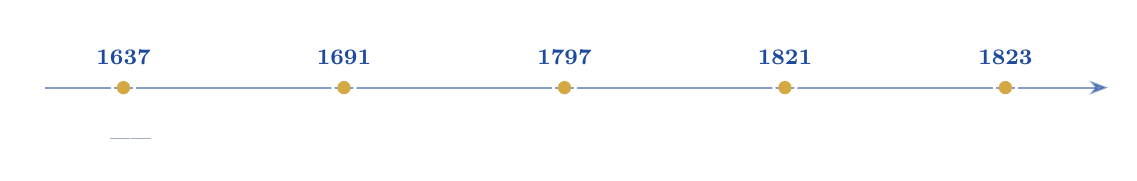
\begin{tikzpicture}[x=1cm,y=1cm,>=Stealth]
  % 主轴
  \draw[->,thick,deepblue,opacity=0.55] (0.5,0) -- (14.0,0);
  % 五个里程碑
  \foreach \x/\yr/\thm/\book in {
    1.5/1637/费马定理/{《求最大值和最小值的方法》\\ 极值点切线水平——思想萌芽},
    4.3/1691/罗尔定理/{《方程的解法》\\ 多项式的原始版本},
    7.1/1797/拉格朗日中值定理/{《解析函数论》\\ 首次一般表述},
    9.9/1821/分析严格化/{《分析教程》\\ 极限理论奠基},
    12.7/1823/柯西中值定理/{《无穷小计算教程》\\ 现代形式的证明}} {
    \fill[gold] (\x,0) circle (2.4pt);
    \draw[white,line width=1.1pt] (\x,0) circle (4pt);
    \node[anchor=south,align=center] at (\x,0.16)
      {\fontsize{8}{9}\selectfont\heiti\bfseries\color{deepblue}\yr};
    \node[anchor=south,align=center,text width=2.2cm] at (\x,0.52)
      {\fontsize{7.4}{8.4}\selectfont\heiti\bfseries\color{ncblue}\thm};
    \node[anchor=north,align=center,text width=2.2cm] at (\x,-0.16)
      {\fontsize{6.2}{7.2}\selectfont\color{muted}\book};
  }
\end{tikzpicture}
\end{center}
\vskip2pt
\begin{tcolorbox}[fgold]
\flabelg{史料视角}
{\fontsize{7.8}{9.4}\selectfont\sloppy 罗尔 1691 年的原始表述只针对\textbf{多项式}；我们今天看到的微分中值定理体系，由拉格朗日（1797）与柯西（1823）接力完成；中值定理的两百年旅程，正是微积分\textbf{严密化}的缩影。\par}
\end{tcolorbox}
\end{frame}

% ============================================================ 推广链
\begin{frame}{一条主线 · 从特殊到一般}
\vskip6pt
\begin{center}
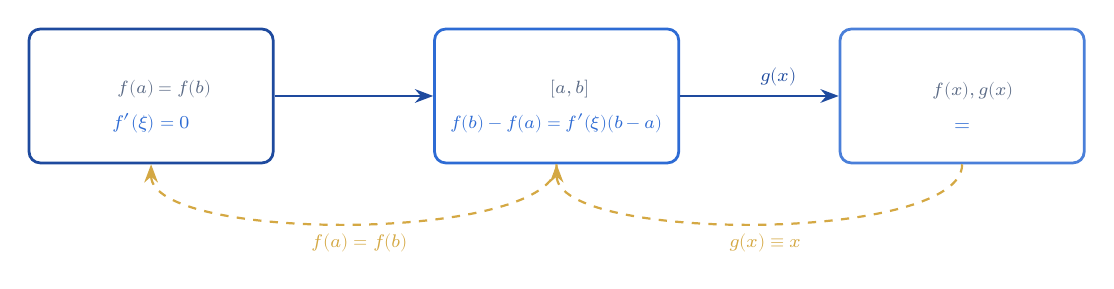
\begin{tikzpicture}[x=1cm,y=1cm,>=Stealth,font=\small]
  % 三个定理盒
  \node[fill=white,draw=deepblue,line width=1pt,rounded corners=4pt,minimum width=3.1cm,minimum height=1.7cm,align=center,text=ink] (r) at (2.0,2.0)
    {{\fontsize{9}{10}\selectfont\heiti\bfseries\color{deepblue}罗尔定理}\\[1.5pt]{\fontsize{6.4}{7.4}\selectfont\color{muted}端点等值 \(f(a)=f(b)\)}\\[1.5pt]{\fontsize{6.6}{7.6}\selectfont\color{ncblue}\(f'(\xi)=0\)}};
  \node[fill=white,draw=ncblue,line width=1pt,rounded corners=4pt,minimum width=3.1cm,minimum height=1.7cm,align=center,text=ink] (l) at (7.15,2.0)
    {{\fontsize{9}{10}\selectfont\heiti\bfseries\color{ncblue}拉格朗日中值定理}\\[1.5pt]{\fontsize{6.4}{7.4}\selectfont\color{muted}一般区间 \([a,b]\)}\\[1.5pt]{\fontsize{6.4}{7.4}\selectfont\color{ncblue}\(f(b)-f(a)=f'(\xi)(b-a)\)}};
  \node[fill=white,draw=accent,line width=1pt,rounded corners=4pt,minimum width=3.1cm,minimum height=1.7cm,align=center,text=ink] (c) at (12.3,2.0)
    {{\fontsize{9}{10}\selectfont\heiti\bfseries\color{accent}柯西中值定理}\\[1.5pt]{\fontsize{6.4}{7.4}\selectfont\color{muted}双函数 \(f(x),g(x)\)}\\[1.5pt]{\fontsize{6.4}{7.4}\selectfont\color{accent}增量比 = 导数比}};
  % 上箭头：一般化
  \draw[->,thick,deepblue] (r.east) -- (l.west)
    node[midway,above,font=\fontsize{6.6}{7.6}\selectfont\heiti\color{deepblue}]{取消端点等值};
  \draw[->,thick,deepblue] (l.east) -- (c.west)
    node[midway,above,font=\fontsize{6.6}{7.6}\selectfont\heiti\color{deepblue}]{引入参数函数 \(g(x)\)};
  % 下箭头：特殊化（金色）
  \draw[->,thick,dashed,gold] (c.south) .. controls +(0,-1.0) and +(0,-1.0) .. (l.south)
    node[midway,below,font=\fontsize{6.6}{7.6}\selectfont\heiti\color{golddeep}]{令 \(g(x)\equiv x\)};
  \draw[->,thick,dashed,gold] (l.south) .. controls +(0,-1.0) and +(0,-1.0) .. (r.south)
    node[midway,below,font=\fontsize{6.6}{7.6}\selectfont\heiti\color{golddeep}]{令 \(f(a)=f(b)\)};
\end{tikzpicture}
\end{center}
\vskip1pt
\begin{tcolorbox}[fgold]
\flabelg{学法建议}
{\fontsize{7.8}{9.4}\selectfont 学定理要学会“两头走”：\textbf{往上一般化}——看清定理的威力边界；\textbf{往下特殊化}——用特例验证一般结论的真身。进可攻，退可守。}
\end{tcolorbox}
\end{frame}

% ============================================================ 章节页 02
\sectdiv{02}{定理内涵}{ROLLE · LAGRANGE · CAUCHY}{2}

% ============================================================ 罗尔定理内容
\begin{frame}{罗尔定理 · 内容与条件}
\begin{theobox}{罗尔定理（Rolle）}
设函数 \(f(x)\) 满足：
\begin{enumerate}
  \item 在闭区间 \([a,b]\) 上\textbf{连续}；
  \item 在开区间 \((a,b)\) 内\textbf{可导}；
  \item \(f(a)=f(b)\)（\textbf{端点等值}）。
\end{enumerate}
则至少存在一点 \(\xi\in(a,b)\)，使得\quad \(f'(\xi)=0\)。
\end{theobox}
\vskip4pt
\begin{columns}[c,onlytextwidth]
\column{0.32\textwidth}\condcard{1}{闭连续 · 曲线连绵}
\column{0.32\textwidth}\condcard{2}{开可导 · 切线存在}
\column{0.32\textwidth}\condcard{3}{端等值 · 首尾同高}
\end{columns}
\vskip5pt
\begin{tcolorbox}[fgold]
\flabelg{记忆口诀}
{\fontsize{8.2}{9.6}\selectfont “\textbf{闭连 · 开导 · 端等值}”——三把钥匙缺一不可。首尾等高的光滑曲线，在峰谷之处切线必水平。}
\end{tcolorbox}
\end{frame}

% ============================================================ 罗尔定理几何直观
\begin{frame}{罗尔定理 · 几何直观}
\begin{columns}[c,onlytextwidth]
\column{0.50\textwidth}
\begin{center}
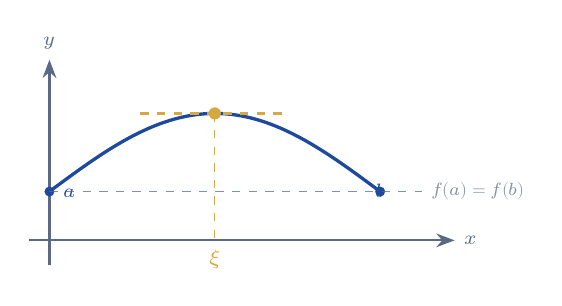
\begin{tikzpicture}[x=1.05cm,y=0.62cm,>=Stealth]
  \draw[->,thick,muted] (-0.25,0) -- (4.9,0) node[right,font=\fontsize{7}{8}\selectfont]{$x$};
  \draw[->,thick,muted] (0,-0.5) -- (0,3.7) node[above,font=\fontsize{7}{8}\selectfont]{$y$};
  % 曲线：首尾等高、中间一峰
  \draw[very thick,deepblue,domain=0:4,samples=100,smooth] plot (\x,{1+1.6*sin(45*\x)});
  % 端点
  \fill[deepblue] (0,1) circle (1.8pt);
  \fill[deepblue] (4,1) circle (1.8pt);
  \node[font=\fontsize{7}{8}\selectfont\color{deepblue},anchor=south west] at (0.05,0.68) {$a$};
  \node[font=\fontsize{7}{8}\selectfont\color{deepblue},anchor=south] at (4,0.68) {$b$};
  % 端等值虚线
  \draw[dashed,muted,opacity=0.75] (0,1) -- (4.5,1)
    node[right,font=\fontsize{6.4}{7.4}\selectfont\color{muted}]{$f(a)=f(b)$};
  % 峰点与水平切线
  \coordinate (P) at (2,2.6);
  \fill[gold] (P) circle (2.2pt);
  \draw[dashed,gold] (P) -- (2,0) node[below,font=\fontsize{7.5}{8.5}\selectfont\color{golddeep}]{$\xi$};
  \draw[dashed,very thick,gold] (1.1,2.6) -- (2.9,2.6)
    node[right,font=\fontsize{6.6}{7.6}\selectfont\heiti\color{golddeep}]{水平切线};
\end{tikzpicture}
\end{center}
\column{0.47\textwidth}
\pointcard{代数语言}{\(f'(\xi)=0\) 的几何身份就是“切线水平”——定理把代数条件翻译成了图形特征。}
\pointcard{物理类比}{竖直上抛的小球：整段行程的平均速度为 0，必有一瞬间（最高点）瞬时速度为 0。}
\pointcard{认知提醒}{峰、谷、驻点都可以是 \(\xi\) 的藏身处——\(\xi\) 存在，但未必唯一。}
\end{columns}
\end{frame}

% ============================================================ 缺一不可
\begin{frame}{罗尔定理 · 条件“缺一不可”}
\begin{columns}[c,onlytextwidth]
\column{0.32\textwidth}
\begin{center}
{\fontsize{8}{9.2}\selectfont\heiti\bfseries\color{deepblue}条件一 · 不连续~{\color{warnred}$\times$}}\\[3pt]
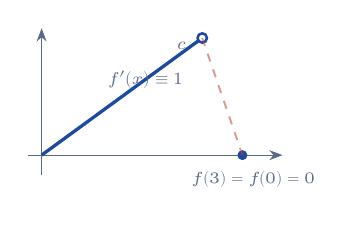
\begin{tikzpicture}[x=0.85cm,y=0.62cm,>=Stealth]
  \draw[->,muted] (-0.2,0) -- (3.6,0);
  \draw[->,muted] (0,-0.4) -- (0,2.6);
  \draw[very thick,deepblue] (0,0) -- (2.4,2.4);
  \fill[white,draw=deepblue,line width=0.9pt] (2.4,2.4) circle (1.7pt);
  \fill[deepblue] (3,0) circle (1.8pt);
  \draw[dashed,warnred,opacity=0.55,line width=0.7pt] (2.4,2.4) -- (3,0);
  \node[font=\fontsize{6.2}{7.2}\selectfont\color{muted},anchor=west] at (0.85,1.55) {\(f'(x)\equiv1\)};
  \node[font=\fontsize{6.2}{7.2}\selectfont\color{muted},anchor=north east] at (2.3,2.52) {间断于点 \(c\)};
  \node[font=\fontsize{5.8}{6.8}\selectfont\color{muted},anchor=north] at (3,-0.14) {端值相等：\(f(3)=f(0)=0\)};
\end{tikzpicture}
\end{center}
\column{0.32\textwidth}
\begin{center}
{\fontsize{8}{9.2}\selectfont\heiti\bfseries\color{deepblue}条件二 · 不可导~{\color{warnred}$\times$}}\\[3pt]
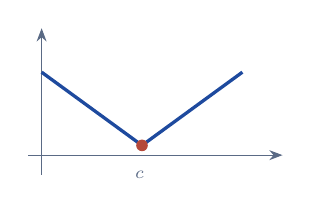
\begin{tikzpicture}[x=0.85cm,y=0.62cm,>=Stealth]
  \draw[->,muted] (-0.2,0) -- (3.6,0);
  \draw[->,muted] (0,-0.4) -- (0,2.6);
  \draw[very thick,deepblue] (0,1.7) -- (1.5,0.2) -- (3,1.7);
  \fill[warnred] (1.5,0.2) circle (2.1pt);
  \node[font=\fontsize{6.2}{7.2}\selectfont\color{muted},anchor=north] at (1.5,-0.12) {尖点 \(c\) 不可导};
\end{tikzpicture}
\end{center}
\column{0.32\textwidth}
\begin{center}
{\fontsize{8}{9.2}\selectfont\heiti\bfseries\color{deepblue}条件三 · 端不等值~{\color{warnred}$\times$}}\\[3pt]
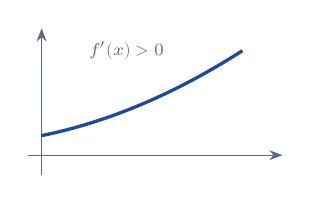
\begin{tikzpicture}[x=0.85cm,y=0.62cm,>=Stealth]
  \draw[->,muted] (-0.2,0) -- (3.6,0);
  \draw[->,muted] (0,-0.4) -- (0,2.6);
  \draw[very thick,deepblue,domain=0:3,samples=60,smooth] plot (\x,{0.4+0.28*\x+0.1*\x*\x});
  \node[font=\fontsize{6.2}{7.2}\selectfont\color{muted},anchor=south] at (1.5,1.75) {\(f'(x)>0\) 无水平切线};
\end{tikzpicture}
\end{center}
\end{columns}
\vskip8pt
\begin{tcolorbox}[fgold]
\flabelg{课堂思考}
{\fontsize{7.8}{9.4}\selectfont 三个条件任何一条被突破，结论都可能“塌方”。反过来想一想：如果曲线有\textbf{多个峰谷}，满足 \(f'(\xi)=0\) 的点会有几个？（\(\xi\) 的存在性 ≠ 唯一性）}
\end{tcolorbox}
\end{frame}

% ============================================================ 拉格朗日中值定理内容
\begin{frame}{拉格朗日中值定理 · 内容}
\begin{theobox}{拉格朗日中值定理（Lagrange）}
设函数 \(f(x)\) 满足：
\begin{enumerate}
  \item 在闭区间 \([a,b]\) 上连续；
  \item 在开区间 \((a,b)\) 内可导。
\end{enumerate}
则至少存在一点 \(\xi\in(a,b)\)，使得\quad \(f(b)-f(a)=f'(\xi)\,(b-a)\)。
\end{theobox}
\vskip4pt
\begin{tcolorbox}[fcard]
\flabel{有限增量公式}
\[\Delta y=f(x+\Delta x)-f(x)=f'(x+\theta\,\Delta x)\,\Delta x,\qquad 0<\theta<1\]
\end{tcolorbox}
\vskip4pt
\begin{tcolorbox}[fgold]
\flabelg{条件升级与本质}
{\fontsize{7.8}{9.4}\selectfont 与罗尔定理相比，“端点等值”的限制被\textbf{取消}；函数的\textbf{整体增量}被某点的\textbf{瞬时变化率}精确表达——连接“局部”与“整体”的第一座桥梁。}
\end{tcolorbox}
\end{frame}

% ============================================================ 拉格朗日几何直观
\begin{frame}{拉格朗日中值定理 · 几何直观}
\begin{columns}[c,onlytextwidth]
\column{0.50\textwidth}
\begin{center}
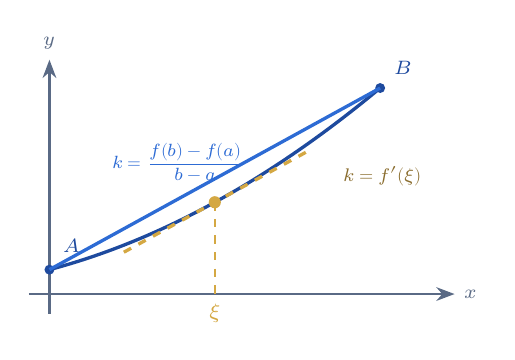
\begin{tikzpicture}[x=1.05cm,y=0.62cm,>=Stealth]
  \draw[->,thick,muted] (-0.25,0) -- (4.9,0) node[right,font=\fontsize{7}{8}\selectfont]{$x$};
  \draw[->,thick,muted] (0,-0.4) -- (0,4.8) node[above,font=\fontsize{7}{8}\selectfont]{$y$};
  % 一般弧线
  \draw[very thick,deepblue,domain=0:4,samples=100,smooth] plot (\x,{0.5+0.45*\x+0.12*\x*\x});
  % 端点与弦
  \fill[deepblue] (0,0.5) circle (1.8pt);
  \fill[deepblue] (4,4.22) circle (1.8pt);
  \node[font=\fontsize{7}{8}\selectfont\color{deepblue},anchor=south west] at (0.05,0.66) {$A$};
  \node[font=\fontsize{7}{8}\selectfont\color{deepblue},anchor=south west] at (4.06,4.3) {$B$};
  \draw[very thick,ncblue] (0,0.5) -- (4,4.22);
  \node[font=\fontsize{6.4}{7.4}\selectfont\heiti\color{ncblue},anchor=south] at (1.5,2.12)
    {弦：\(k=\dfrac{f(b)-f(a)}{b-a}\)};
  % 平行切线
  \coordinate (M) at (2,1.88);
  \fill[gold] (M) circle (2.2pt);
  \draw[dashed,very thick,gold] (0.9,0.857) -- (3.1,2.903);
  \draw[dashed,gold,line width=0.7pt] (M) -- (2,0) node[below,font=\fontsize{7.5}{8.5}\selectfont\color{golddeep}]{$\xi$};
  \node[font=\fontsize{6.6}{7.6}\selectfont\heiti\color{golddeep},anchor=west] at (3.25,2.42)
    {切线：\(k=f'(\xi)\)};
\end{tikzpicture}
\end{center}
\column{0.47\textwidth}
\pointcard{几何语言}{曲线上至少有一点的切线\textbf{平行于弦} \(AB\)——“以直代曲”的精确版。}
\pointcard{运动学语言}{整段行程的\textbf{平均速率}，必被某一时刻的\textbf{瞬时速率}命中。}
\pointcard{分析语言}{\[\Delta y=f'(\xi)\,\Delta x\] 微分 \(\mathrm{d}y=f'(x)\Delta x\) 只是近似，中值定理给出\textbf{精确等式}。}
\end{columns}
\end{frame}

% ============================================================ 两个推论
\begin{frame}{两个推论 · 导数的“归零”与“对齐”}
\begin{columns}[c,onlytextwidth]
\column{0.49\textwidth}
\begin{corobox}{导数恒为零，函数恒为常数}
若 \(f'(x)\equiv0\)（区间 \(I\) 内），则 \(f(x)\) 在 \(I\) 上恒为常数。
\vskip2pt
{\fontsize{7}{8.6}\selectfont\color{muted}\textbf{证明线索：}任取 \(x_1<x_2\)，由拉格朗日中值定理 \(f(x_2)-f(x_1)=f'(\xi)(x_2-x_1)=0\)。}
\end{corobox}
\column{0.49\textwidth}
\begin{corobox}{导数恒相等，函数差常数}
若 \(f'(x)\equiv g'(x)\)（区间 \(I\) 内），则 \(f(x)=g(x)+C\)。
\vskip2pt
{\fontsize{7}{8.6}\selectfont\color{muted}\textbf{证明线索：}对 \(F(x)=f(x)-g(x)\) 应用推论 1。}
\end{corobox}
\end{columns}
\vskip7pt
\begin{tcolorbox}[fgold]
\flabelg{方法预告 · 证明恒等式“三步法”}
{\fontsize{8.2}{9.8}\selectfont
\numsq{ncblue}{1}~构造：令 \(F(x)=\text{左}-\text{右}\)\qquad
\numsq{ncblue}{2}~证零：\(F'(x)\equiv0\)，由推论 1 得 \(F\equiv C\)\qquad
\numsq{ncblue}{3}~定值：取特殊点求出 \(C\)}
\end{tcolorbox}
\vskip5pt
{\fontsize{7.6}{9.2}\selectfont\color{muted}随堂快问：若 \(f'(x)>0\) 恒成立，\(f(x)\) 是否单调递增？（提示：推论 2 保证“两个可导函数若导数相同则只差常数”）}
\end{frame}

% ============================================================ 柯西中值定理内容
\begin{frame}{柯西中值定理 · 内容}
\begin{theobox}{柯西中值定理（Cauchy）}
设函数 \(f(x)\) 与 \(g(x)\) 满足：
\begin{enumerate}
  \item 在闭区间 \([a,b]\) 上连续；
  \item 在开区间 \((a,b)\) 内可导；
  \item 对任意 \(x\in(a,b)\)，\(g'(x)\ne0\)。
\end{enumerate}
则至少存在一点 \(\xi\in(a,b)\)，使得
\[\frac{f(b)-f(a)}{g(b)-g(a)}=\frac{f'(\xi)}{g'(\xi)}.\]
\end{theobox}
\vskip4pt
\begin{columns}[c,onlytextwidth]
\column{0.49\textwidth}
\begin{tcolorbox}[fgold]
\flabelg{条件警示}
{\fontsize{7.6}{9}\selectfont 条件 (3) 保证 \(g(b)-g(a)\ne0\)（分母不为零）——这是柯西定理的“专属条款”，用时千万别漏！}
\end{tcolorbox}
\column{0.49\textwidth}
\pointcard{本质解读}{两个函数“增量比”的中点形态——把拉格朗日定理中的自变量 \(x\)，换成用另一个函数 \(g(x)\) 来度量。}
\end{columns}
\end{frame}

% ============================================================ 柯西几何解释
\begin{frame}{柯西中值定理 · 参数曲线解释}
\begin{columns}[c,onlytextwidth]
\column{0.50\textwidth}
\begin{center}
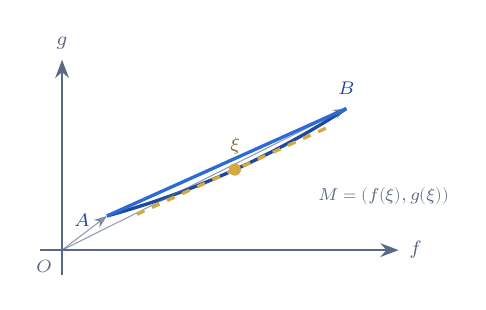
\begin{tikzpicture}[x=0.95cm,y=0.62cm,>=Stealth]
  \draw[->,thick,muted] (-0.3,0) -- (4.5,0) node[right,font=\fontsize{7}{8}\selectfont]{$f$};
  \draw[->,thick,muted] (0,-0.5) -- (0,3.9) node[above,font=\fontsize{7}{8}\selectfont]{$g$};
  \node[font=\fontsize{6.4}{7.4}\selectfont\color{muted},anchor=north east] at (0,0) {$O$};
  % 参数曲线弧 A→B
  \draw[very thick,deepblue] (0.6,0.7) .. controls (1.8,1.2) and (2.9,2.0) .. (3.8,2.9);
  % 位置矢量
  \draw[->,thin,muted,opacity=0.65] (0,0) -- (0.6,0.7);
  \draw[->,thin,muted,opacity=0.65] (0,0) -- (3.8,2.9);
  % 弦
  \draw[very thick,ncblue] (0.6,0.7) -- (3.8,2.9);
  % 平行切线
  \coordinate (M) at (2.31,1.65);
  \fill[gold] (M) circle (2.2pt);
  \draw[dashed,very thick,gold] (1.0,0.734) -- (3.6,2.549);
  % 标注
  \node[font=\fontsize{6.6}{7.6}\selectfont\color{deepblue},anchor=east] at (0.5,0.62) {$A$};
  \node[font=\fontsize{6.6}{7.6}\selectfont\color{deepblue},anchor=south] at (3.8,2.98) {$B$};
  \node[font=\fontsize{6.6}{7.6}\selectfont\color{golddeep},anchor=south] at (2.31,1.76) {$\xi$};
  \node[font=\fontsize{6.4}{7.4}\selectfont\color{ncblue},anchor=west] at (0.9,-0.42) {弦};
  \node[font=\fontsize{6.4}{7.4}\selectfont\color{golddeep},anchor=west] at (3.05,-0.42) {切线};
  \node[font=\fontsize{6.2}{7.2}\selectfont\color{muted},anchor=west] at (3.3,1.1) {$M=(f(\xi),g(\xi))$};
\end{tikzpicture}
\end{center}
\column{0.47\textwidth}
\pointcard{弹性标尺}{横坐标不再匀速前进——\(g(x)\) 像一把\textbf{会弯曲的尺子}，按自己的节奏丈量弧上点的位置。}
\pointcard{弦切平行}{参数曲线 \(x=f(t),\,y=g(t)\) 的弧上，必有一点的切线\textbf{平行于弦} \(AB\)。}
\pointcard{特例回落}{取 \(g(x)=x\)，柯西定理立刻退回\textbf{拉格朗日中值定理}——它是拉格朗日定理的“参数化升级”。}
\end{columns}
\end{frame}

% ============================================================ 三定理关系图
\begin{frame}{一图看懂 · 三大中值定理的逻辑}
\begin{center}
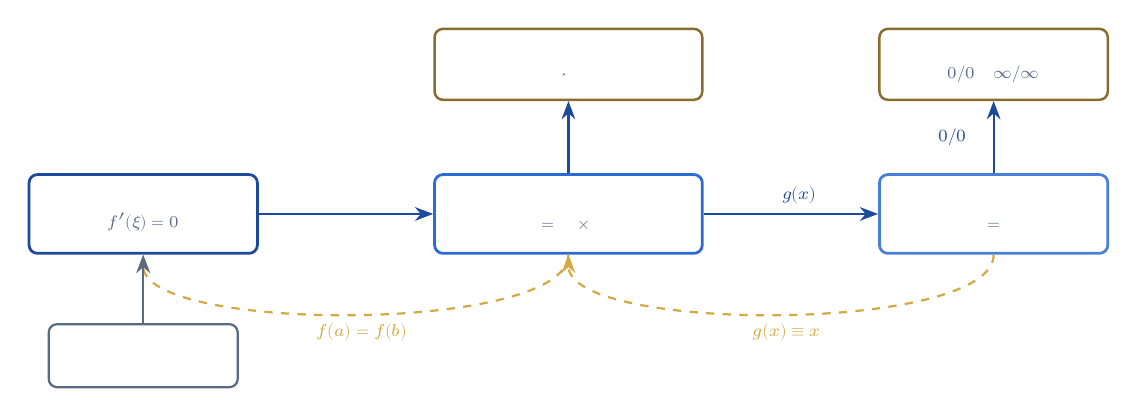
\begin{tikzpicture}[x=1cm,y=1cm,>=Stealth,font=\small]
  % 底层：费马定理
  \node[fill=white,draw=muted,line width=0.8pt,rounded corners=3pt,minimum width=2.4cm,minimum height=0.8cm,align=center] (f) at (2.4,0.5)
    {{\fontsize{8}{9}\selectfont\heiti\bfseries\color{ink}费马定理}\\[0.5pt]{\fontsize{5.8}{6.8}\selectfont\color{muted}极值点导数为零}};
  % 中层三定理
  \node[fill=white,draw=deepblue,line width=1pt,rounded corners=3pt,minimum width=2.9cm,minimum height=1.0cm,align=center] (r) at (2.4,2.3)
    {{\fontsize{8.6}{9.6}\selectfont\heiti\bfseries\color{deepblue}罗尔定理}\\[0.5pt]{\fontsize{6}{7}\selectfont\color{muted}\(f'(\xi)=0\)}};
  \node[fill=white,draw=ncblue,line width=1pt,rounded corners=3pt,minimum width=3.4cm,minimum height=1.0cm,align=center] (l) at (7.8,2.3)
    {{\fontsize{8.6}{9.6}\selectfont\heiti\bfseries\color{ncblue}拉格朗日中值定理}\\[0.5pt]{\fontsize{6}{7}\selectfont\color{muted}增量 \(=\) 导数 \(\times\) 区间长}};
  \node[fill=white,draw=accent,line width=1pt,rounded corners=3pt,minimum width=2.9cm,minimum height=1.0cm,align=center] (c) at (13.2,2.3)
    {{\fontsize{8.6}{9.6}\selectfont\heiti\bfseries\color{accent}柯西中值定理}\\[0.5pt]{\fontsize{6}{7}\selectfont\color{muted}增量比 \(=\) 导数比}};
  % 上层：泰勒公式 / 洛必达法则
  \node[fill=white,draw=golddeep,line width=0.9pt,rounded corners=3pt,minimum width=3.4cm,minimum height=0.9cm,align=center] (t) at (7.8,4.2)
    {{\fontsize{8.6}{9.6}\selectfont\heiti\bfseries\color{golddeep}泰勒公式}\\[0.5pt]{\fontsize{6}{7}\selectfont\color{muted}高阶推广 · 拉格朗日余项}};
  \node[fill=white,draw=golddeep,line width=0.9pt,rounded corners=3pt,minimum width=2.9cm,minimum height=0.9cm,align=center] (h) at (13.2,4.2)
    {{\fontsize{8.6}{9.6}\selectfont\heiti\bfseries\color{golddeep}洛必达法则}\\[0.5pt]{\fontsize{6}{7}\selectfont\color{muted}\(0/0\) 与 \(\infty/\infty\)}};
  % 蓝色：一般化方向
  \draw[->,thick,deepblue] (r.east) -- (l.west)
    node[midway,above,font=\fontsize{6.2}{7.2}\selectfont\heiti\color{deepblue}]{取消端等值};
  \draw[->,thick,deepblue] (l.east) -- (c.west)
    node[midway,above,font=\fontsize{6.2}{7.2}\selectfont\heiti\color{deepblue}]{引入 \(g(x)\)};
  % 金色虚线：特殊化方向
  \draw[->,thick,dashed,gold] (c.south) .. controls +(0,-1.0) and +(0,-1.0) .. (l.south)
    node[midway,below,font=\fontsize{6.2}{7.2}\selectfont\heiti\color{golddeep}]{令 \(g(x)\equiv x\)};
  \draw[->,thick,dashed,gold] (l.south) .. controls +(0,-1.0) and +(0,-1.0) .. (r.south)
    node[midway,below,font=\fontsize{6.2}{7.2}\selectfont\heiti\color{golddeep}]{令 \(f(a)=f(b)\)};
  % 纵向联系
  \draw[->,thick,deepblue] (l.north) -- (t.south)
    node[midway,right,font=\fontsize{6.2}{7.2}\selectfont\heiti\color{deepblue}]{高阶推广};
  \draw[->,thick,deepblue] (c.north) -- (h.south)
    node[midway,left,font=\fontsize{6.2}{7.2}\selectfont\heiti\color{deepblue}]{\(0/0\) 基石};
  \draw[->,thick,muted] (f.north) -- (r.south)
    node[midway,left,font=\fontsize{6.2}{7.2}\selectfont\heiti\color{muted}]{理论基石};
\end{tikzpicture}
\end{center}
\vskip1pt
\begin{tcolorbox}[fgold]
\flabelg{全局视野}
{\fontsize{7.8}{9.4}\selectfont 三大定理是一条\textbf{推广链}；向上长出泰勒公式，向下引出洛必达法则——一张网，撑起微分学的半壁江山。}
\end{tcolorbox}
\end{frame}

% ============================================================ 章节页 03
\sectdiv{03}{应用探究}{FIVE CLASSIC APPLICATIONS}{3}

% ============================================================ 应用一 · 不等式
\begin{frame}{应用一 · 证明不等式}
\begin{tcolorbox}[fgold]
\flabelg{方法三板斧}
{\fontsize{7.8}{9.4}\selectfont \textbf{选函数}（把结论凑成 \(f(b)-f(a)\) 的形状）\(\to\) \textbf{套定理}（拉格朗日中值定理）\(\to\) \textbf{放缩}（估计 \(|f'(\xi)|\) 的上界）\hfill\tagpill{考研数学 · 高频题型}}
\end{tcolorbox}
\vskip4pt
\begin{columns}[c,onlytextwidth]
\column{0.32\textwidth}\appcard{\(\ln x\le x-1\ (x>0)\)}{\(f(t)=\ln t\) 于 \([1,x]\)}{\(\frac1\xi\le1\)（\(x>1\)）}
\column{0.32\textwidth}\appcard{\(e^x\ge 1+x\ (x\ge0)\)}{\(f(t)=e^t\) 于 \([0,x]\)}{\(e^\xi>1\)}
\column{0.32\textwidth}\appcard{\(|\arctan u-\arctan v|\le|u-v|\)}{\(f(t)=\arctan t\) 于 \([u,v]\)}{\(|f'(\xi)|\le1\)}
\end{columns}
\vskip5pt
\begin{exambox}{证明 \(e^x\ge 1+x\)（\(x\ge0\)）}
\(x=0\) 时取等号。当 \(x>0\) 时，对 \(f(t)=e^t\) 在 \([0,x]\) 上应用拉格朗日中值定理：
\[e^x-1=e^{\xi}\,x,\qquad \xi\in(0,x).\]
因 \(\xi>0\) 时 \(e^\xi>1\)，故 \(e^x-1>x\)，即 \(e^x>1+x\)。综上所证。
\end{exambox}
\end{frame}

% ============================================================ 应用二 · 恒等式
\begin{frame}{应用二 · 证明恒等式}
\begin{exambox}{证明 \(\arcsin x+\arccos x=\dfrac{\pi}{2}\)（\(-1\le x\le1\)）}
设 \(F(x)=\arcsin x+\arccos x\)。在 \((-1,1)\) 内，
\[F'(x)=\frac{1}{\sqrt{1-x^2}}-\frac{1}{\sqrt{1-x^2}}\equiv 0.\]
由\textbf{推论 1}，\(F(x)\equiv C\)。令 \(x=0\) 得 \(C=F(0)=0+\dfrac{\pi}{2}=\dfrac{\pi}{2}\)；又 \(F\) 在 \([\,-1,1]\) 上连续，端点处亦成立，所证等式成立。
\end{exambox}
\vskip4pt
\begin{tcolorbox}[htmlcard,title={\iconsq{gold}{法}\hspace{7pt}证明恒等式“三步法”}]
{\fontsize{7.8}{9.4}\selectfont
\numsq{ncblue}{1}~构造：令 \(F(x)=\text{左}-\text{右}\)\quad
\numsq{ncblue}{2}~证零：证 \(F'(x)\equiv0\)，由推论 1 得 \(F\equiv C\)\quad
\numsq{ncblue}{3}~定值：取特殊点（如 \(x=0\)）求出 \(C\)}
\end{tcolorbox}
\end{frame}

% ============================================================ 应用三 · 方程根
\begin{frame}{应用三 · 方程根的存在性与唯一性}
\begin{exambox}{证明方程 \(x^3+x-1=0\) 有且只有一个实根}
\textbf{（1）存在性}：设 \(f(x)=x^3+x-1\)，则 \(f(x)\) 在 \(\mathbb{R}\) 上连续，且
\[f(0)=-1<0,\qquad f(1)=1>0.\]
由零点定理，\(f(x)\) 在 \((0,1)\) 内至少有一个零点，即方程\textbf{至少有一个}实根。

\textbf{（2）唯一性}：反设方程有两个实根 \(x_1<x_2\)，则 \(f(x_1)=f(x_2)=0\)，且 \(f(x)\) 在 \([x_1,x_2]\) 上可导。由\textbf{罗尔定理}，存在 \(\xi\in(x_1,x_2)\) 使 \(f'(\xi)=0\)。但
\[f'(x)=3x^2+1>0\quad(\text{恒成立}),\]
矛盾。故方程\textbf{至多有一个}实根。

综合（1）（2）：方程 \(x^3+x-1=0\) 有且只有一个实根。
\end{exambox}
\vskip4pt
\begin{tcolorbox}[fgold]
\flabelg{解题套路}
{\fontsize{7.8}{9.4}\selectfont “有且仅有一个根”两步走：\textbf{存在性}靠零点定理，\textbf{唯一性}靠罗尔定理反证——导数恒正（或恒负）\(\Rightarrow\) 至多一根。}
\end{tcolorbox}
\end{frame}

% ============================================================ 应用四 · 洛必达
\begin{frame}{应用四 · 洛必达法则的理论基石}
\begin{tcolorbox}[fgold]
\flabelg{推导 · 柯西中值定理出手}
{\fontsize{7.4}{9}\selectfont 设 \(f(a)=g(a)=0\)，\(g'(x)\ne0\)。对 \(f,g\) 于 \([a,x]\) 上应用\textbf{柯西中值定理}：
\[\frac{f(x)}{g(x)}=\frac{f(x)-f(a)}{g(x)-g(a)}=\frac{f'(\xi)}{g'(\xi)},\qquad \xi\in(a,x).\]
令 \(x\to a\) 则 \(\xi\to a\)，若右端极限存在，即得
\[\lim_{x\to a}\frac{f(x)}{g(x)}=\lim_{x\to a}\frac{f'(x)}{g'(x)}.\]
由此得到\textbf{洛必达法则（\(0/0\) 型）}：\(\lim f=\lim g=0\) 且 \(\lim f'/g'\) 存在时，\(\lim\dfrac{f}{g}=\lim\dfrac{f'}{g'}\)（\(\infty/\infty\) 型同理）。}
\end{tcolorbox}
\vskip4pt
\begin{exambox}{洛必达求极限}
取 \(f=e^x-1-x\)，\(g=x^2\)：\(\lim\limits_{x\to0}\dfrac{e^x-1-x}{x^2}=\lim\limits_{x\to0}\dfrac{e^x-1}{2x}=\lim\limits_{x\to0}\dfrac{e^x}{2}=\dfrac12\)。
\end{exambox}
\vskip3pt
{\fontsize{7.2}{8.8}\selectfont\color{muted}\textbf{警示：}用前必验 \(0/0\) 或 \(\infty/\infty\)；每次求导后重新验算；\(\lim f'/g'\) 不存在不可断言原极限不存在。}
\end{frame}

% ============================================================ 应用五 · 泰勒公式
\begin{frame}{应用五 · 泰勒公式——高阶中值定理}
\begin{columns}[c,onlytextwidth]
\column{0.44\textwidth}
\begin{center}
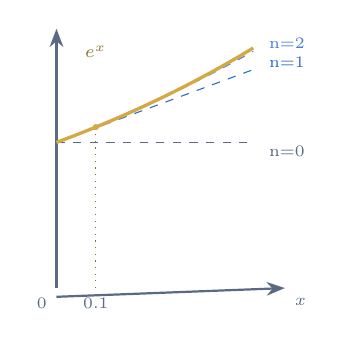
\begin{tikzpicture}[x=5.0cm,y=1.85cm,>=Stealth]
  \draw[->,thick,muted] (0,-0.06) -- (0.58,0) node[anchor=north west,font=\fontsize{6}{7}\selectfont]{$x$};
  \draw[->,thick,muted] (0,0) -- (0,1.78);
  \node[anchor=north east,font=\fontsize{5.8}{6.6}\selectfont\color{muted}] at (0,0) {0};
  \node[anchor=north,font=\fontsize{5.8}{6.6}\selectfont\color{muted}] at (0.1,0) {0.1};
  \draw[dotted,golddeep] (0.1,0) -- (0.1,1.1052);
  \fill[gold] (0.1,1.1052) circle (1.1pt);
  \draw[dashed,muted] (0,1) -- (0.5,1);
  \draw[dashed,ncblue] (0,1) -- (0.5,1.5);
  \draw[dashed,accent,domain=0:0.5,samples=40] plot (\x,{1+\x+\x*\x/2});
  \draw[very thick,gold,domain=0:0.5,samples=60,smooth] plot (\x,{exp(\x)});
  \node[anchor=west,font=\fontsize{5.8}{6.6}\selectfont\heiti\color{muted}] at (0.515,0.94) {n=0};
  \node[anchor=west,font=\fontsize{5.8}{6.6}\selectfont\heiti\color{ncblue}] at (0.515,1.55) {n=1};
  \node[anchor=west,font=\fontsize{5.8}{6.6}\selectfont\heiti\color{accent}] at (0.515,1.68) {n=2};
  \node[anchor=west,font=\fontsize{6.4}{7.2}\selectfont\heiti\bfseries\color{golddeep}] at (0.05,1.62) {$e^x$};
\end{tikzpicture}
\end{center}
\column{0.53\textwidth}
\begin{tcolorbox}[fcard]
\flabel{泰勒公式（带拉格朗日余项）}
\[f(x)=\sum_{k=0}^{n}\frac{f^{(k)}(x_0)}{k!}(x-x_0)^k\]
\[\qquad+\frac{f^{(n+1)}(\xi)}{(n+1)!}(x-x_0)^{n+1}\]
{\fontsize{7.8}{9.4}\selectfont\(\xi\) 介于 \(x_0\) 与 \(x\) 之间；\(n=0\) 时即拉格朗日定理。}
\end{tcolorbox}
\vskip4pt
\begin{exambox}{近似计算 \(e^{0.1}\)}
取 \(n=2\)：\(e^{0.1}\approx 1+0.1+\dfrac{0.1^2}{2!}=1.105\)，误差 \(|R_2|\le\dfrac{e^{0.1}\cdot 0.1^3}{3!}<2\times10^{-4}\)。
\end{exambox}
\end{columns}
\end{frame}

% ============================================================ 综合实战
\begin{frame}{综合实战 · 辅助函数的构造艺术}
\begin{exambox}{证明存在 \(\xi\)，使 \(\dfrac{b\,f(b)-a\,f(a)}{b-a}=f(\xi)+\xi f'(\xi)\)}
设 \(f(x)\) 在 \([a,b]\) 上连续、\((a,b)\) 内可导，且 \(a>0\)。

\textbf{分析（破题）}：结论右端 \(=f(\xi)+\xi f'(\xi)=\bigl[x f(x)\bigr]'_{x=\xi}\)，正是 \(F(x)=x f(x)\) 在 \(\xi\) 处的导数；左端恰是 \(F\) 在 \([a,b]\) 上的“平均变化率”——结论就是拉格朗日中值定理的\textbf{现成形态}。

\textbf{证明}：令 \(F(x)=x f(x)\)，则 \(F(x)\) 在 \([a,b]\) 上连续、\((a,b)\) 内可导。由拉格朗日中值定理，存在 \(\xi\in(a,b)\)，使得
\[F(b)-F(a)=F'(\xi)(b-a),\]
即 \(b\,f(b)-a\,f(a)=\bigl[f(\xi)+\xi f'(\xi)\bigr](b-a)\)。得证。
\end{exambox}
\vskip4pt
\begin{tcolorbox}[htmlcard,title={\iconsq{gold}{造}\hspace{7pt}构造三步法与“原料库”}]
{\fontsize{7.6}{9.2}\selectfont
\textbf{三步法：}盯结论（识别“像谁的导数”）\(\to\) 造函数 \(\to\) 套定理（验条件、下结论）。\par\vskip2pt
\textbf{原料库：}结论含 \(x f(x)\) \(\to\) 造 \(F=xf(x)\)；含 \(e^{\lambda x}f(x)\) \(\to\) 造 \(F=e^{\lambda x}f(x)\)；含 \(\dfrac{f(x)}{x}\) \(\to\) 造 \(F=\dfrac{f(x)}{x}\)。\hfill\tagpill{考研经典 · 构造法}}
\end{tcolorbox}
\end{frame}

% ============================================================ 章节页 04
\sectdiv{04}{方法提升}{FROM THEOREMS TO METHODS}{4}

% ============================================================ 知识结构图
\begin{frame}{知识结构图 · 一章一网}
\begin{center}
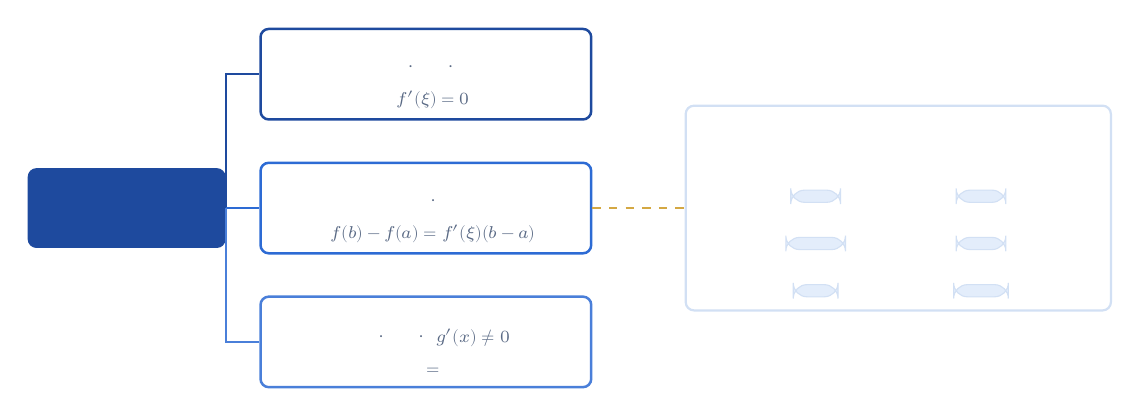
\begin{tikzpicture}[x=1cm,y=1cm,>=Stealth,font=\small]
  % 根
  \node[fill=deepblue,draw=deepblue,rounded corners=3pt,minimum width=2.5cm,minimum height=1.0cm,align=center,text=white] (root) at (1.2,2.8)
    {{\fontsize{9}{10}\selectfont\heiti\bfseries 微分中值定理}\\[0.5pt]{\fontsize{6}{7}\selectfont 导数应用的纲}};
  % 三个分支
  \node[fill=white,draw=deepblue,line width=0.9pt,rounded corners=3pt,minimum width=4.2cm,minimum height=1.15cm,align=center] (b1) at (5.0,4.5)
    {{\fontsize{8.4}{9.4}\selectfont\heiti\bfseries\color{deepblue}罗尔定理}\\[1pt]{\fontsize{6.2}{7.4}\selectfont\color{muted}条件：闭连 · 开导 · 端等值}\\[0.5pt]{\fontsize{6.2}{7.4}\selectfont\color{muted}结论：\(f'(\xi)=0\)}};
  \node[fill=white,draw=ncblue,line width=0.9pt,rounded corners=3pt,minimum width=4.2cm,minimum height=1.15cm,align=center] (b2) at (5.0,2.8)
    {{\fontsize{8.4}{9.4}\selectfont\heiti\bfseries\color{ncblue}拉格朗日中值定理}\\[1pt]{\fontsize{6.2}{7.4}\selectfont\color{muted}条件：闭连 · 开导}\\[0.5pt]{\fontsize{6.2}{7.4}\selectfont\color{muted}结论：\(f(b)-f(a)=f'(\xi)(b-a)\)}};
  \node[fill=white,draw=accent,line width=0.9pt,rounded corners=3pt,minimum width=4.2cm,minimum height=1.15cm,align=center] (b3) at (5.0,1.1)
    {{\fontsize{8.4}{9.4}\selectfont\heiti\bfseries\color{accent}柯西中值定理}\\[1pt]{\fontsize{6.2}{7.4}\selectfont\color{muted}条件：闭连 · 开导 · \(g'(x)\ne0\)}\\[0.5pt]{\fontsize{6.2}{7.4}\selectfont\color{muted}结论：增量比 \(=\) 导数比}};
  % 右侧应用地图（大盒 + 6 个小标签节点，不用嵌套小图）
  \node[fill=white,draw=cborder,line width=0.8pt,rounded corners=3pt,minimum width=5.4cm,minimum height=2.6cm] (app) at (11.0,2.8) {};
  \node[font=\fontsize{8.4}{9.4}\selectfont\heiti\bfseries\color{deepblue}] at (11.0,3.62) {应用地图};
  \node[fill=titlebg,draw=cborder,line width=0.4pt,rounded corners=5pt,inner xsep=4.5pt,inner ysep=2.2pt] at (9.95,2.95) {\fontsize{6.4}{7.2}\selectfont\heiti\color{ncblue}证明不等式};
  \node[fill=titlebg,draw=cborder,line width=0.4pt,rounded corners=5pt,inner xsep=4.5pt,inner ysep=2.2pt] at (12.05,2.95) {\fontsize{6.4}{7.2}\selectfont\heiti\color{ncblue}证明恒等式};
  \node[fill=titlebg,draw=cborder,line width=0.4pt,rounded corners=5pt,inner xsep=4.5pt,inner ysep=2.2pt] at (9.95,2.35) {\fontsize{6.4}{7.2}\selectfont\heiti\color{ncblue}方程根的存在性};
  \node[fill=titlebg,draw=cborder,line width=0.4pt,rounded corners=5pt,inner xsep=4.5pt,inner ysep=2.2pt] at (12.05,2.35) {\fontsize{6.4}{7.2}\selectfont\heiti\color{ncblue}洛必达法则};
  \node[fill=titlebg,draw=cborder,line width=0.4pt,rounded corners=5pt,inner xsep=4.5pt,inner ysep=2.2pt] at (9.95,1.75) {\fontsize{6.4}{7.2}\selectfont\heiti\color{ncblue}泰勒近似};
  \node[fill=titlebg,draw=cborder,line width=0.4pt,rounded corners=5pt,inner xsep=4.5pt,inner ysep=2.2pt] at (12.05,1.75) {\fontsize{6.4}{7.2}\selectfont\heiti\color{ncblue}构造辅助函数};
  % 连线
  \draw[thick,deepblue] (root.east) |- (b1.west);
  \draw[thick,ncblue] (root.east) |- (b2.west);
  \draw[thick,accent] (root.east) |- (b3.west);
  \draw[thick,dashed,gold] (b2.east) -- (app.west);
\end{tikzpicture}
\end{center}
\vskip2pt
\begin{tcolorbox}[fgold]
\flabelg{思想主线}
{\fontsize{7.8}{9.4}\selectfont 几何直观 \(\to\) 严格表述 \(\to\) 相互推广 \(\to\) 场景应用——学一章，拎一条线。}
\end{tcolorbox}
\end{frame}

% ============================================================ 易错辨析
\begin{frame}{易错辨析 · 四个“坑”}
\begin{columns}[c,onlytextwidth]
\column{0.49\textwidth}
\warncard{坑一 · \(\xi\) 未必唯一}{定理只承诺“\textbf{至少一个}”。多峰曲线可以命中多个 \(\xi\)；且 \(\xi\) 的具体值通常求不出，也不需要求出。}
\column{0.49\textwidth}
\warncard{坑二 · \(\xi\) 在开区间}{\(\xi\in(a,b)\) 而非 \([a,b]\)——端点处 \(f'(a)\)、\(f'(b)\) 未必存在，把 \(\xi\) 写成端点是常见笔误。}
\end{columns}
\vskip5pt
\begin{columns}[c,onlytextwidth]
\column{0.49\textwidth}
\warncard{坑三 · 条件必须验齐}{三条“高压线”：闭连续 / 开可导 / 端等值（罗尔）或 \(g'(x)\ne0\)（柯西）。缺任何一条，结论都可能失效。}
\column{0.49\textwidth}
\warncard{坑四 · 分母不能为零}{柯西定理靠 \(g'(x)\ne0\) 保证 \(g(b)\ne g(a)\)；洛必达每次求导后，都要重新检验是否仍为 \(0/0\) 或 \(\infty/\infty\)。}
\end{columns}
\vskip7pt
\begin{tcolorbox}[fgold]
\flabelg{用定理前默念三句话}
{\fontsize{8}{9.4}\selectfont 条件验齐没有？\(\xi\) 写在开区间没有？分母、极限验算没有？}
\end{tcolorbox}
\end{frame}

% ============================================================ 分层作业与评价量规
\begin{frame}{分层作业 · 评价量规}
\begin{columns}[c,onlytextwidth]
\column{0.56\textwidth}
\tierbox{\iconsq{ncblue}{基}\hspace{6pt}基础 · 必做}{%
{\fontsize{7}{8.6}\selectfont
\textbf{1.}\ 验证罗尔定理对 \(f(x)=x^3-x\) 在 \([-1,1]\) 上的正确性，并找出所有的 \(\xi\)。\par\vskip1.5pt
\textbf{2.}\ 证明不等式：\(|\sin x_1-\sin x_2|\le |x_1-x_2|\)。\par\vskip1.5pt
\textbf{3.}\ 证明：当 \(x>1\) 时，\(e^x>e\,x\)。}}
\vskip3pt
\tierbox{\iconsq{deepblue}{提}\hspace{6pt}提高 · 选做}{%
{\fontsize{7}{8.6}\selectfont
\textbf{4.}\ 证明恒等式：当 \(x>0\) 时，\(\arctan x+\arctan\tfrac1x=\tfrac{\pi}{2}\)。\par\vskip1.5pt
\textbf{5.}\ 设 \(f\) 在 \([0,1]\) 上连续、\((0,1)\) 内可导，且 \(f(0)=0,\ f(1)=1\)。证明：对任意正整数 \(n\)，存在 \(\xi\in(0,1)\)，使 \(f'(\xi)=n\xi^{n-1}\)。\ \ {\color{muted}（提示：对 \(f\) 与 \(g(x)=x^n\) 用柯西中值定理）}}}
\column{0.41\textwidth}
\tierbox{\iconsq{gold}{拓}\hspace{6pt}拓展 · 挑战}{%
{\fontsize{7}{8.6}\selectfont
\textbf{6.}\ 证明：当 \(0<b<a\) 时，\(\dfrac{a-b}{a}<\ln\dfrac{a}{b}<\dfrac{a-b}{b}\)。\ \ {\color{muted}（提示：对 \(f(x)=\ln x\) 于 \([b,a]\) 用拉格朗日中值定理）}}}
\vskip3pt
\begin{tcolorbox}[htmlcard,title={\iconsq{deepblue}{评}\hspace{7pt}评价量规（Rubric）}]
{\fontsize{6.2}{7.6}\selectfont
\begin{tabular}{@{}p{1.0cm}p{2.3cm}p{0.55cm}@{}}
{\heiti\bfseries\color{deepblue}维度} & {\heiti\bfseries\color{deepblue}观测点} & {\heiti\bfseries\color{deepblue}权重}\\
概念理解 & 陈述条件结论会画图 & 30\%\\
定理应用 & 验条件选定理，规范写 & 40\%\\
构造思想 & 识别原料构造辅助函数 & 20\%\\
反思表达 & 错题归因清晰多解 & 10\%\\
\end{tabular}}
\vskip2pt
{\fontsize{6.4}{7.8}\selectfont\color{muted}订正要求：错题归因“漏验 / 构造 / 计算”三类，课前 5 分钟互评。}
\end{tcolorbox}
\end{columns}
\end{frame}

 

\end{document}
